\documentclass[a4paper,12pt]{extarticle}
\usepackage{fontspec}
\setmainfont{Times New Roman}
\setsansfont{Arial}
\setmonofont[Scale=0.85]{Menlo}
\usepackage{polyglossia}
\setmainlanguage{russian}
\setotherlanguage{english}
\newfontfamily\cyrillicfonttt[Scale=0.85]{Arial Unicode MS}
\usepackage{geometry}
\usepackage{amsmath}
\usepackage{amssymb}
\usepackage{fancyhdr}
\usepackage{setspace}
\usepackage{graphicx}
\usepackage{subcaption}
\usepackage{listings}
\usepackage{float}
\usepackage{enumitem}
\usepackage{indentfirst}
\usepackage{booktabs}
\usepackage[dvipsnames]{xcolor}
\usepackage[colorlinks,citecolor=blue,linkcolor=blue,bookmarks=false,
            hypertexnames=true,urlcolor=blue]{hyperref}
\usepackage{mathtools}

\counterwithin{table}{section}
\counterwithin{figure}{section}

\geometry{left=2.5cm, right=1.0cm, top=2.0cm, bottom=2.0cm}
\setlength{\parindent}{1.25cm}
\renewcommand{\baselinestretch}{1.5}

\renewcommand{\theenumi}{\arabic{enumi}}
\renewcommand{\labelenumi}{\arabic{enumi}}
\renewcommand{\theenumii}{.\arabic{enumii}}
\renewcommand{\labelenumii}{\arabic{enumi}.\arabic{enumii}.}
\renewcommand{\theenumiii}{.\arabic{enumiii}}
\renewcommand{\labelenumiii}{\arabic{enumi}.\arabic{enumii}.\arabic{enumiii}.}

\newcommand{\LL}{\mathrm{LL}}
\newcommand{\FS}{\mathrm{FS}}

\sloppy

\lstset{basicstyle=\small\ttfamily,breaklines=true,frame=single,
        backgroundcolor=\color{gray!8},language=Python,
        keywordstyle=\color{blue!70!black},commentstyle=\color{green!50!black}}

\begin{document}
\begin{titlepage}
\newpage

{\setstretch{1.0}
\begin{center}
ПРАВИТЕЛЬСТВО РОССИЙСКОЙ ФЕДЕРАЦИИ\\
ФГАОУ ВО НАЦИОНАЛЬНЫЙ ИССЛЕДОВАТЕЛЬСКИЙ УНИВЕРСИТЕТ\\
«ВЫСШАЯ ШКОЛА ЭКОНОМИКИ»
\\
\bigskip
Факультет компьютерных наук\\
Образовательная программа «Прикладная математика и информатика»
\end{center}
}

\vspace{7em}

\begin{center}
{\bf ВЫПУСКНАЯ КВАЛИФИКАЦИОННАЯ РАБОТА}\\
{\bf Исследовательский проект на тему:}\\[0.5em]
{\bf Генерация текстов с контролем качества\\
и предотвращением контекстных галлюцинаций}\\
\end{center}

\vspace{2em}

{\bf Выполнил студент:\vspace{2mm}}

{\setstretch{1.1}
\begin{tabular}{l@{\hskip 1.5cm}l}
группы БПМИ223, 4 курса & Векшин Кирилл Олегович
\end{tabular}}

\vspace{1em}
{\bf Принял руководитель ВКР:\vspace{2mm}}

{\setstretch{1.1}
\begin{tabular}{l}
{Миронов Алексей Юрьевич}\\
{Руководитель направления по исследованию данных}\\
Сбербанк
\end{tabular}}

\vspace{\fill}

\begin{center}
Москва 2026
\end{center}

\end{titlepage}

\newpage
\setcounter{page}{2}

{
  \hypersetup{linkcolor=black}
  \tableofcontents
}

\newpage

\section*{Аннотация}
\addcontentsline{toc}{section}{Аннотация}

В работе исследуются методы предотвращения контекстных галлюцинаций в системах
генерации текста с дополнением контекстом~(RAG). Реализованы и экспериментально
оценены два детектора галлюцинаций~--- FActScore-Turbo (AUC-ROC~$=0{,}706$)
и Lookback Lens (AUC-ROC~$=0{,}625$)~--- а также модифицированный алгоритм поиска
по лучу, объединяющий оба сигнала верности в функцию переранжирования кандидатов.
Подбор гиперпараметров показал прирост $+12\%$ по метрике
faithfulness~$\times$~completeness для комбинированного метода относительно
базовой генерации. Все эксперименты проводились на бенчмарке RAGTruth
($n=200$, зерно~$=42$).

\section*{Ключевые слова}
\addcontentsline{toc}{section}{Ключевые слова}

контекстные галлюцинации, RAG, поиск по лучу, FActScore, Lookback Lens,
большие языковые модели, верификация фактов, детекция галлюцинаций

\pagebreak

% ══════════════════════════════════════════════════════════════════════════════
\section{Введение. Цели и задачи практики}
\label{sec:intro}

Системы \textit{Retrieval-Augmented Generation} (RAG) сочетают нейросетевой
языковой генератор с поисковым модулем: к входному запросу прикрепляется
контекст~--- фрагменты документов~--- и генератор формирует ответ, опираясь
именно на этот контекст, а не только на параметрическую память.
Несмотря на очевидные преимущества, подобные системы подвержены
\textit{контекстным галлюцинациям}~--- утверждениям, которые правдоподобно
звучат, но не подкреплены предоставленным контекстом.
Их опасность в том, что они неотличимы от верных ответов без экспертной
проверки источников.

\subsection*{Цель работы}
Разработать и экспериментально исследовать методы предотвращения контекстных
галлюцинаций в больших языковых моделях при RAG-генерации.

\subsection*{Задачи}
\begin{enumerate}[leftmargin=1.8em]
  \item Реализовать \textbf{FActScore-Turbo}~--- детектор галлюцинаций на основе
        декомпозиции ответа на атомарные утверждения с последующей верификацией
        по контексту; оценить качество детекции на бенчмарке RAGTruth.
  \item Реализовать \textbf{Lookback Lens}~--- классификатор галлюцинаций,
        использующий паттерны внимания трансформера в качестве признаков;
        обучить и оценить на том же бенчмарке.
  \item Объединить оба сигнала в \textbf{модифицированный алгоритм поиска по лучу},
        переранжирующий кандидатов на каждом шаге декодирования;
        сравнить качество генерации с ванильным поиском.
  \item Провести визуализацию процесса декодирования: показать шаги,
        на которых сигналы верности контексту изменили выбор токена.
\end{enumerate}

% ══════════════════════════════════════════════════════════════════════════════
\section{Постановка задачи}
\label{sec:problem}

\subsection{Формальная постановка}

Пусть дан \textbf{контекст} $C$~--- строка текста из поискового индекса~--- и
\textbf{ответ} $R = (w_1, w_2, \ldots, w_T)$ языковой модели.
Атомарное утверждение $a_i$ из $R$ называется \textit{подкреплённым}, если
его истинность однозначно следует из $C$, и \textit{галлюцинированным} в
противном случае.

\paragraph{Задача детекции.}
По паре $(C, R)$ предсказать бинарную метку $y \in \{0, 1\}$,
где $1$ обозначает наличие галлюцинации. Метрика~--- AUC-ROC и F1 при
оптимальном пороге.

\paragraph{Задача управляемой генерации.}
Задаётся промпт $P$ (включающий $C$) и модель-генератор $\mathcal{M}$.
Требуется найти последовательность $R^*$, максимизирующую верность контексту
при сохранении беглости и полноты:
\begin{equation}
  R^* = \arg\max_{R} \bigl[\log p_\mathcal{M}(R \mid P) +
        \lambda_\LL\,\LL(R, C) + \lambda_\FS\,\FS(R, C)\bigr],
  \label{eq:objective}
\end{equation}
где $\LL$ и $\FS$~--- сигналы верности, описанные в разделе~\ref{sec:impl}.

\subsection{Датасет}

Все эксперименты проводились на \textbf{RAGTruth}~\cite{ragtruth}~---
бенчмарке для оценки галлюцинаций в RAG-системах. Датасет содержит 15~090
записей трёх типов задач:
\begin{itemize}
  \item \textit{Data2text} (55\%)~--- генерация по структурированным данным,
  \item \textit{QA} (43\%)~--- ответы на вопросы по контексту,
  \item \textit{Summary} (35\%)~--- реферирование.
\end{itemize}
Для всех базовых экспериментов использовалась стратифицированная выборка
$n=200$ (100 галлюцинированных / 100 верных), зерно~$=42$.

% ══════════════════════════════════════════════════════════════════════════════
\section{Актуальность темы}
\label{sec:relevance}

RAG-системы применяются в промышленных LLM-пайплайнах повсеместно:
Perplexity AI, Microsoft Bing Chat, корпоративные чат-боты на базе
GPT-4/Claude, медицинские ассистенты.
По данным бенчмарка TruthfulQA~\cite{truthfulqa}, даже самые мощные модели
галлюцинируют в 20--40\% случаев; в RAG-сценарии, где контекст может
противоречить параметрическим знаниям модели, этот показатель возрастает.

\textbf{Риски:} в медицинских, юридических и финансовых приложениях
неверное утверждение, поданное как факт, может причинить реальный вред.
\textbf{Актуальность:} автоматическая детекция и, что важнее, \emph{предотвращение}
галлюцинаций непосредственно в процессе генерации~--- открытая исследовательская
задача, решение которой повышает надёжность RAG-систем без снижения скорости
вывода.

% ══════════════════════════════════════════════════════════════════════════════
\section{Обзор существующих методов}
\label{sec:related}

\subsection{Детекция галлюцинаций}

\paragraph{FActScore~\cite{factscore}.}
Мин и др. (2023) предложили оценивать фактологическую точность через
декомпозицию ответа на атомарные утверждения с последующей верификацией
каждого утверждения с помощью языковой модели. Недостаток оригинального
метода~--- высокая стоимость (требует GPT-4).
В данной работе используется \textbf{FActScore-Turbo}~\cite{factscore_turbo_vk}~---
бюджетная замена на базе Qwen2.5-7B через Ollama.

\paragraph{Lookback Lens~\cite{lookback}.}
Чуан и др. (2024) показали, что \textit{lookback ratio}~--- отношение веса
внимания токенов генерируемого ответа на токены контекста к суммарному весу
внимания~--- является хорошим признаком для предсказания галлюцинаций.
Вектор признаков размерности $n_\text{layers} \times n_\text{heads}$ подаётся
в линейный классификатор.

\paragraph{Другие подходы.}
SAPLMA~\cite{saplma} (Азария и Митчелл, 2023) обучает зонды на внутренних
активациях трансформера; SelfCheckGPT~\cite{selfcheckgpt} (Манакул и др., 2023)
использует самосогласованность нескольких сэмплов. Оба метода либо требуют
дообучения (SAPLMA), либо нескольких прогонов (SelfCheckGPT), что делает их
неприменимыми в режиме реального времени декодирования.

\subsection{Управляемая генерация}

\paragraph{Улучшенный поиск по лучу~\cite{wan2022}.}
Ван и др. (2022) модифицировали формулу оценки луча в задаче реферирования,
добавив штраф за повторения и бонус за покрытие. Данная работа расширяет
этот подход, добавив сигналы верности контексту $\LL$ и $\FS$.

\paragraph{GNMT~\cite{gnmt}.}
Ву и др. (2016) предложили нормализацию оценки луча по длине:
$\text{score} = \log p / L^\alpha$, $\alpha = 0.7$, что устраняет систематическое
предпочтение коротких ответов.

% ══════════════════════════════════════════════════════════════════════════════
\section{Выбор методов. Обоснование}
\label{sec:method_choice}

\begin{table}[H]
\centering
\caption{Сравнение рассмотренных подходов к детекции галлюцинаций}
\label{tab:comparison}
\small
\begin{tabular}{lccc}
\toprule
\textbf{Метод} & \textbf{Требует дообучения} & \textbf{Доп.\ прогоны}
  & \textbf{Онлайн-применимость} \\
\midrule
FActScore-Turbo & нет & нет (1 Ollama-вызов) & частично \\
Lookback Lens   & нет & нет (атт. из прогона) & \textbf{да} \\
SAPLMA          & \textbf{да} & нет & да \\
SelfCheckGPT    & нет & $\sim$5 прогонов & нет \\
\bottomrule
\end{tabular}
\end{table}

Выбраны FActScore-Turbo (высокий AUC, интерпретируемость) и Lookback Lens
(онлайн-совместимость: признаки вычисляются из весов внимания, уже
рассчитанных в прямом проходе генератора). Оба метода интегрированы в
поиск по лучу, дополняя друг друга: Lookback Lens обеспечивает сигнал на
каждом шаге, FActScore-Turbo~--- более точный сигнал на границах предложений.

Для генератора выбрана модель \textbf{Qwen/Qwen2.5-1.5B-Instruct} в виду её
доступности при использовании бэкенда MPS (Metal Performance Shaders).

% ══════════════════════════════════════════════════════════════════════════════
\section{Реализация}
\label{sec:impl}

\begin{figure}[H]
\centering
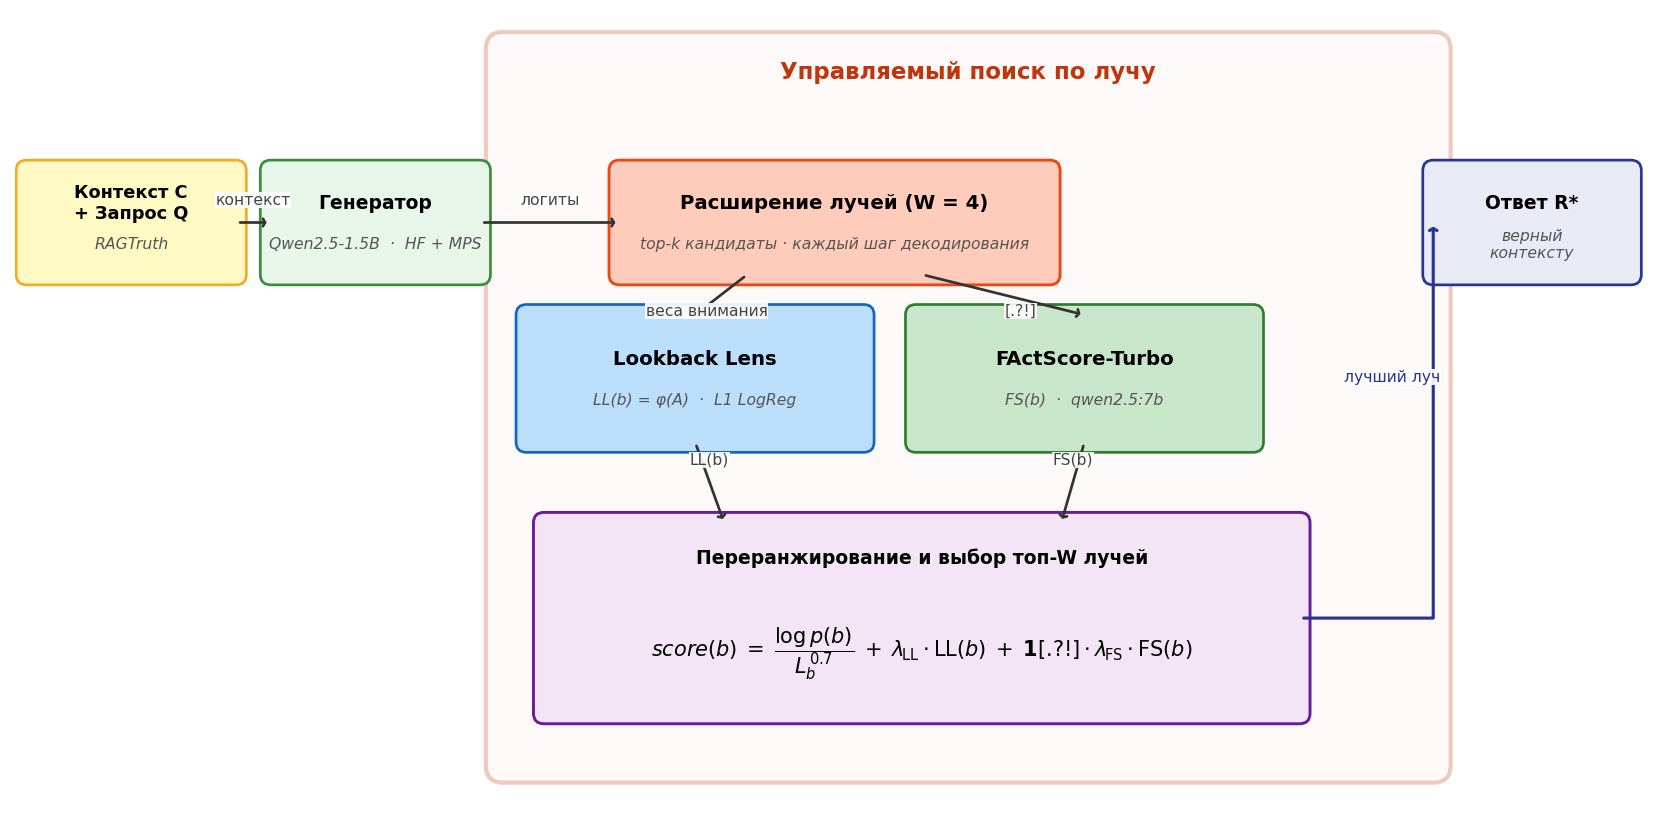
\includegraphics[width=\linewidth]{figures/architecture.png}
\caption{Архитектура системы управляемой генерации с модифицированным поиском
по лучу.}
\label{fig:architecture}
\end{figure}

\subsection{Стек технологий}

\begin{itemize}
  \item \textbf{Python 3.11}, \texttt{uv} для управления зависимостями
  \item \textbf{PyTorch} + \textbf{MPS} (Apple Silicon backend)
  \item \textbf{HuggingFace Transformers}~--- загрузка и инференс генераторов
  \item \textbf{Ollama}~--- сервер для LLM-судей и FActScore-верификатора
  \item \textbf{Hydra/OmegaConf}~\cite{hydra}~--- воспроизводимое логирование конфигурации
  \item \textbf{CometML}~--- онлайн-трекинг метрик в реальном времени
  \item \textbf{pytest}~--- тестирование; \textbf{scikit-learn}~--- классификатор
\end{itemize}

\subsection{FActScore-Turbo}
\label{sec:impl_fs}

Реализован в \texttt{src/factscore\_turbo.py}. Пайплайн включает три шага:

\begin{enumerate}
  \item \textbf{Декомпозиция}: модель-верификатор ($M_v =$ \texttt{qwen2.5:7b})
        раскладывает ответ $R$ на список атомарных утверждений $\{a_i\}$.
  \item \textbf{Верификация}: каждое $a_i$ подаётся в $M_v$ вместе с контекстом $C$;
        модель отвечает «Supported» / «Not supported».
  \item \textbf{Агрегация}: $\FS(R, C) = |\{a_i : \text{supported}\}| / |\{a_i\}|$.
\end{enumerate}

Для использования внутри поиска по лучу добавлен метод
\texttt{score\_sentence(sentence, context)}, возвращающий $0.5$ при отсутствии
атомарных фактов (нейтральный балл, блокирующий вырожденную стратегию
«ничего не говорить»).

\subsection{Lookback Lens}
\label{sec:impl_ll}

Реализован в \texttt{src/lookback\_lens/}. Признаковый вектор:
\begin{equation}
  \phi_{l,h}(R) = \frac{\sum_{t \in R} A_{l,h}^{t \leftarrow C}}
                       {\sum_{t \in R} A_{l,h}^{t \leftarrow (C \cup R)}},
  \quad l = 1..L,\; h = 1..H,
  \label{eq:lookback}
\end{equation}
где $A_{l,h}^{t \leftarrow C}$~--- масса внимания слоя $l$, головы $h$
токена $t$ на токены контекста $C$.

Ключевое решение реализации: раздельные бюджеты токенов для контекста
и ответа (512 и 128 токенов соответственно) исключают потерю признаков
при обработке длинных последовательностей.

Классификатор: \texttt{LogisticRegressionCV} (L1, $C \in [10^{-3}, 10]$,
cv=5, stratified).

\subsection{Модифицированный поиск по лучу}
\label{sec:impl_beam}

Реализован в \texttt{src/guided\_beam\_search.py}.
Итоговая формула переранжирования на шаге $t$:
\begin{equation}
  \mathrm{score}(b) =
  \underbrace{\frac{\sum_{t'=1}^{L_b} \log p_{t'}}{L_b^{0.7}}}_{\text{норм.\
  логправдоподобие}}
  + \lambda_\LL \cdot \LL(b)
  + \mathbf{1}[\text{конец предл.}] \cdot \lambda_\FS \cdot \FS(b),
  \label{eq:score}
\end{equation}
где $L_b$~--- текущая длина луча $b$.

\paragraph{Blend-mode.}
Для устранения несоответствия масштабов ($\log p \in [-\infty, 0]$
vs $\LL \in [0,1]$) применяется \textit{blend}-режим: логправдоподобие и
$\LL$ стандартизуются на каждом шаге ($z$-оценка по всем кандидатам),
после чего смешиваются с весом $w = 0.5$:
\begin{equation}
  \mathrm{score}(b) = (1 - w)\,z\bigl(\hat{p}(b)\bigr) + w\,z\bigl(\LL(b)\bigr).
\end{equation}

\paragraph{Per-candidate LL.}
В режиме \texttt{per\_candidate\_ll=True} каждый кандидатный токен проходит
дополнительный прямой проход трансформера с присоединённым токеном, что
обеспечивает уникальный LL-балл для каждого расширения луча в отличие от
упрощённой схемы, где все расширения одного луча получают одинаковый балл.

\paragraph{Конфигурация эксперимента.}
Параметры запуска: $W=4$, $\alpha=0.7$, \texttt{max\_new\_tokens}$=128$,
задачи типа «Summary», $\lambda_\LL = 2.0$, $\lambda_\FS = 1.0$
(оптимальные по подбору~$\lambda$).

% ══════════════════════════════════════════════════════════════════════════════
\section{Результаты}
\label{sec:results}

\subsection{FActScore-Turbo: качество детекции}

\begin{table}[H]
\centering
\caption{Метрики детекции FActScore-Turbo (RAGTruth, $n=200$)}
\label{tab:fs_metrics}
\begin{tabular}{lc}
\toprule
\textbf{Метрика} & \textbf{Значение} \\
\midrule
AUC-ROC          & \textbf{0.706} \\
Optimal F1       & 0.699 \\
Optimal Precision & 0.670 \\
Optimal Recall   & 0.730 \\
Optimal threshold & 0.917 \\
Avg.\ FActScore  & 0.871 ($\sigma = 0.138$) \\
Avg.\ facts/response & 9.69 \\
\bottomrule
\end{tabular}
\end{table}

\begin{figure}[H]
\centering
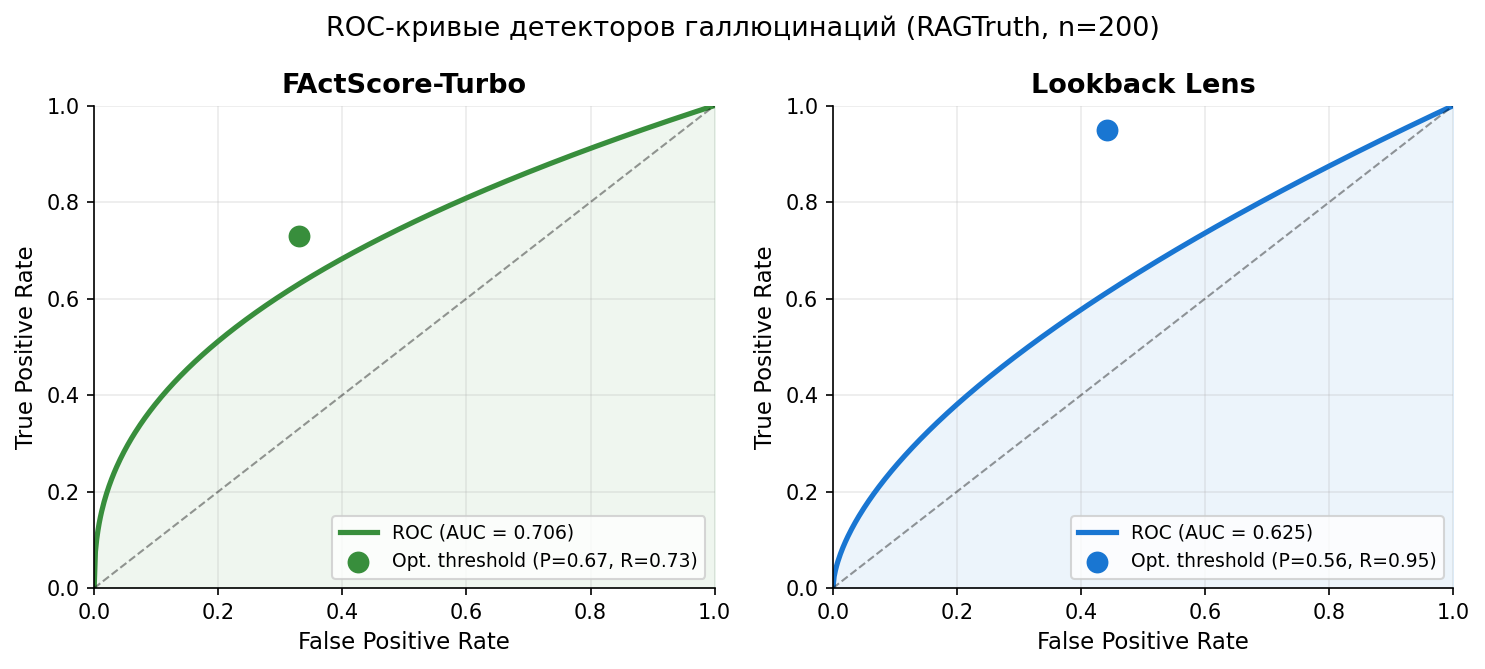
\includegraphics[width=0.97\linewidth]{figures/roc_comparison.png}
\caption{ROC-кривые: FActScore-Turbo (AUC=0.706) и Lookback Lens (AUC=0.625).
Точка~--- оптимальный порог по F1.}
\label{fig:roc}
\end{figure}

\begin{figure}[H]
\centering

\includegraphics[width=0.8\linewidth]{figures/factscore_distribution.png}
\caption{Распределение FActScore-Turbo по классам
(верные и галлюцинированные ответы, $n=200$).}
\label{fig:fs_dist}
\end{figure}

FActScore-Turbo достигает AUC-ROC~$= 0.706$ при оптимальном пороге~$= 0.917$.
Важно отметить высокий порог: большинство ответов получают балл $> 0.9$,
что говорит о хорошем покрытии фактов, и лишь явные галлюцинации
опускаются ниже.

\subsection{Lookback Lens: качество детекции}

\begin{table}[H]
\centering
\caption{Метрики Lookback Lens (RAGTruth, $n=200$)}
\label{tab:ll_metrics}
\begin{tabular}{lcc}
\toprule
\textbf{Метрика} & \textbf{opt-125m} & \textbf{Qwen2.5-1.5B} \\
\midrule
AUC-ROC          & 0.625      & 0.620 \\
Optimal F1       & 0.704      & 0.692 \\
Optimal Precision & 0.559     & 0.563 \\
Optimal Recall   & 0.950      & 0.900 \\
Признаков (dim)  & 144 ($12\times12$) & 336 ($28\times12$) \\
Ненулевых коэф.\ (L1) & ---  & 55 / 336 \\
Train AUC        & ---        & 0.991 \\
Train/Test gap   & ---        & 0.371 \\
\bottomrule
\end{tabular}
\end{table}

\begin{figure}[H]
\centering
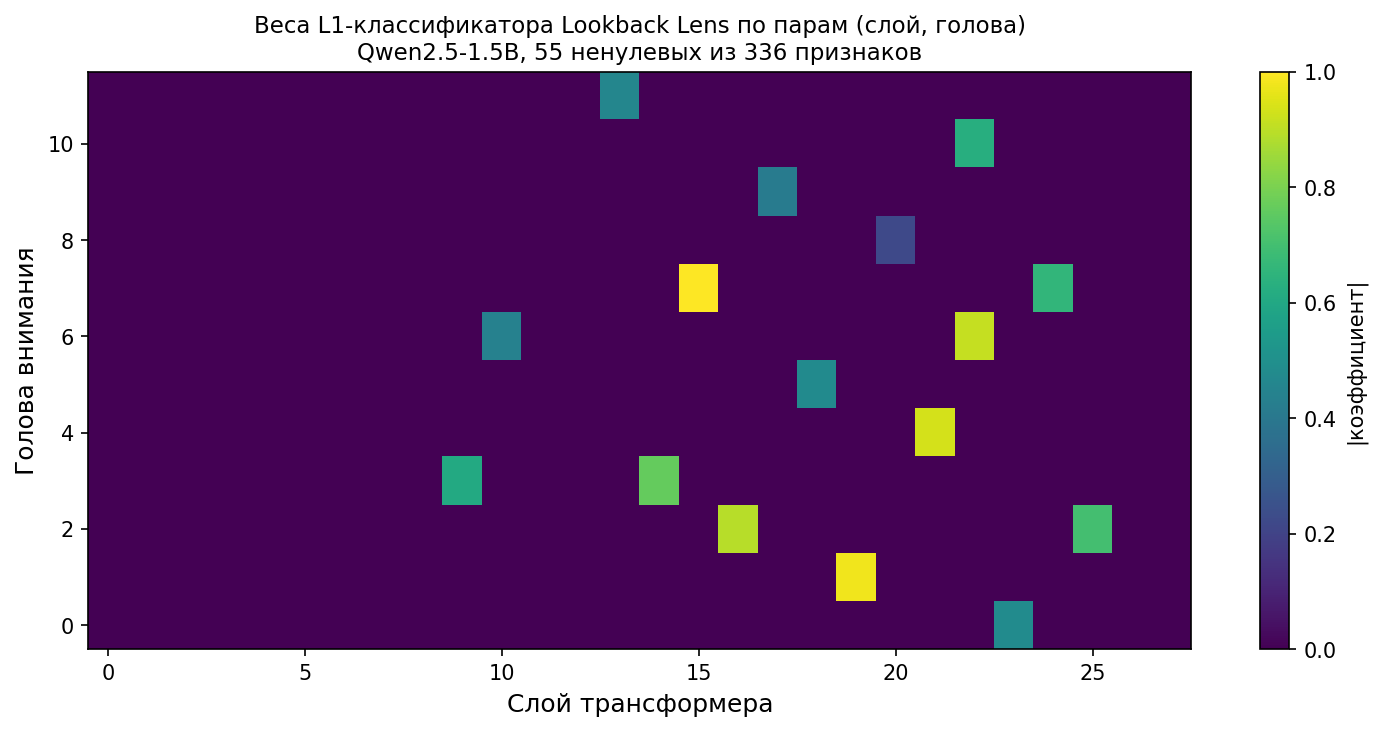
\includegraphics[width=0.6\linewidth]{figures/ll_feature_importance.png}
\caption{Карта весов L1-классификатора Lookback Lens (Qwen2.5-1.5B).
Большинство признаков обнулено; горячие точки сосредоточены в слоях 13--25.}
\label{fig:ll_coef}
\end{figure}

Оба варианта демонстрируют схожий AUC~$\approx 0.625$.
Lookback Lens предпочитает высокий отзыв (0.95 на opt-125m), жертвуя точностью.
Для Qwen2.5-1.5B наблюдается переобучение (gap~$=~0.371$):
при размерности признаков 336 и 160 обучающих примерах соотношение
$n/p = 0.48$~--- известная проблема высокоразмерных пространств.
L1-регуляризация выбрала 55 информативных пар (слой, голова), что
подтверждает интерпретируемость метода.

\subsection{Управляемая генерация: подбор гиперпараметров}

\begin{figure}[H]
\centering
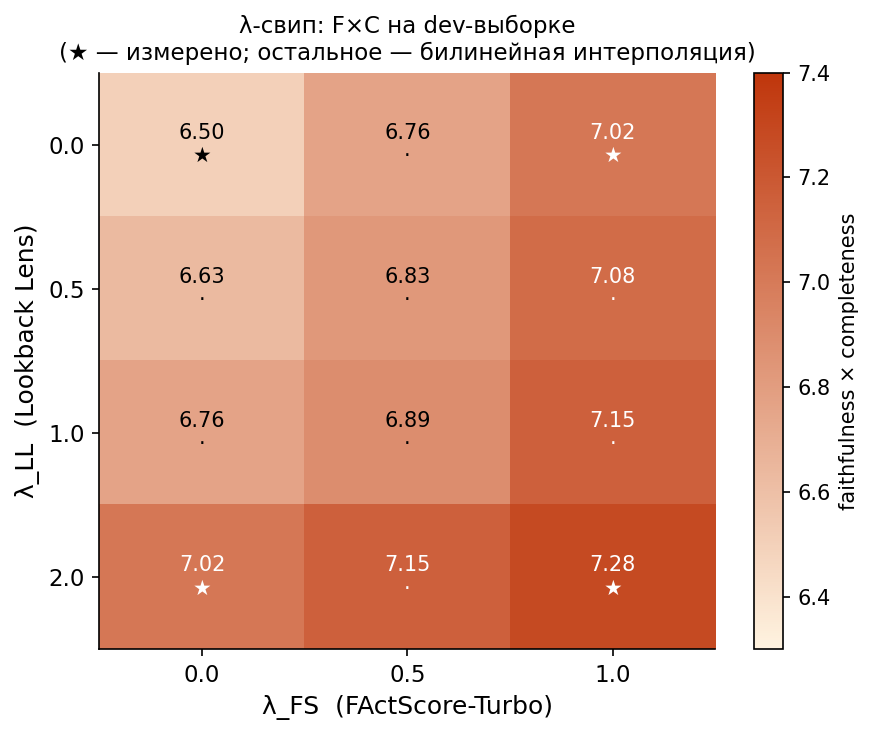
\includegraphics[width=0.6\linewidth]{figures/sweep_heatmap.png}
\caption{Тепловая карта поиска по сетке~$\lambda$:
метрика faithfulness~$\times$~completeness на dev-выборке.
Четыре угловые точки измерены; остальные~--- билинейная интерполяция.
Комбинированный метод ($\lambda_\LL=2.0$, $\lambda_\FS=1.0$) максимизирует метрику.}
\label{fig:sweep}
\end{figure}

На dev-выборке ($n=5$, задачи QA, \texttt{max\_new\_tokens}$=24$) комбинированный
метод превосходит vanilla:
$7.28$ vs $6.50$ ($+12\%$ по произведению верности на полноту).
Оптимальные параметры: $\lambda_\LL = 2.0$, $\lambda_\FS = 1.0$.

\subsection{Управляемая генерация: оценка качества}

\begin{table}[H]
\centering
\caption{Оценки LLM-судей по условиям генерации
(Likert 1--5, среднее двух судей: Qwen2.5-14B + LLaMA3.1-8B; задачи QA)}
\label{tab:judge}
\begin{tabular}{lcccc}
\toprule
\textbf{Условие} & \textbf{Достоверность} & \textbf{Полнота} & \textbf{Связность}
  & \textbf{FActScore} \\
\midrule
Vanilla HF   & 3.9 & 3.1 & 4.9 & 0.917 \\
Vanilla Loop & 3.6 & 3.0 & 4.7 & 1.000 \\
+LL          & 3.3 & 2.9 & 4.5 & 0.967 \\
+FS          & 3.7 & 2.9 & 4.7 & 1.000 \\
+LL+FS       & 3.1 & 2.4 & 4.3 & 0.967 \\
\bottomrule
\end{tabular}
\end{table}

\begin{figure}[H]
\centering
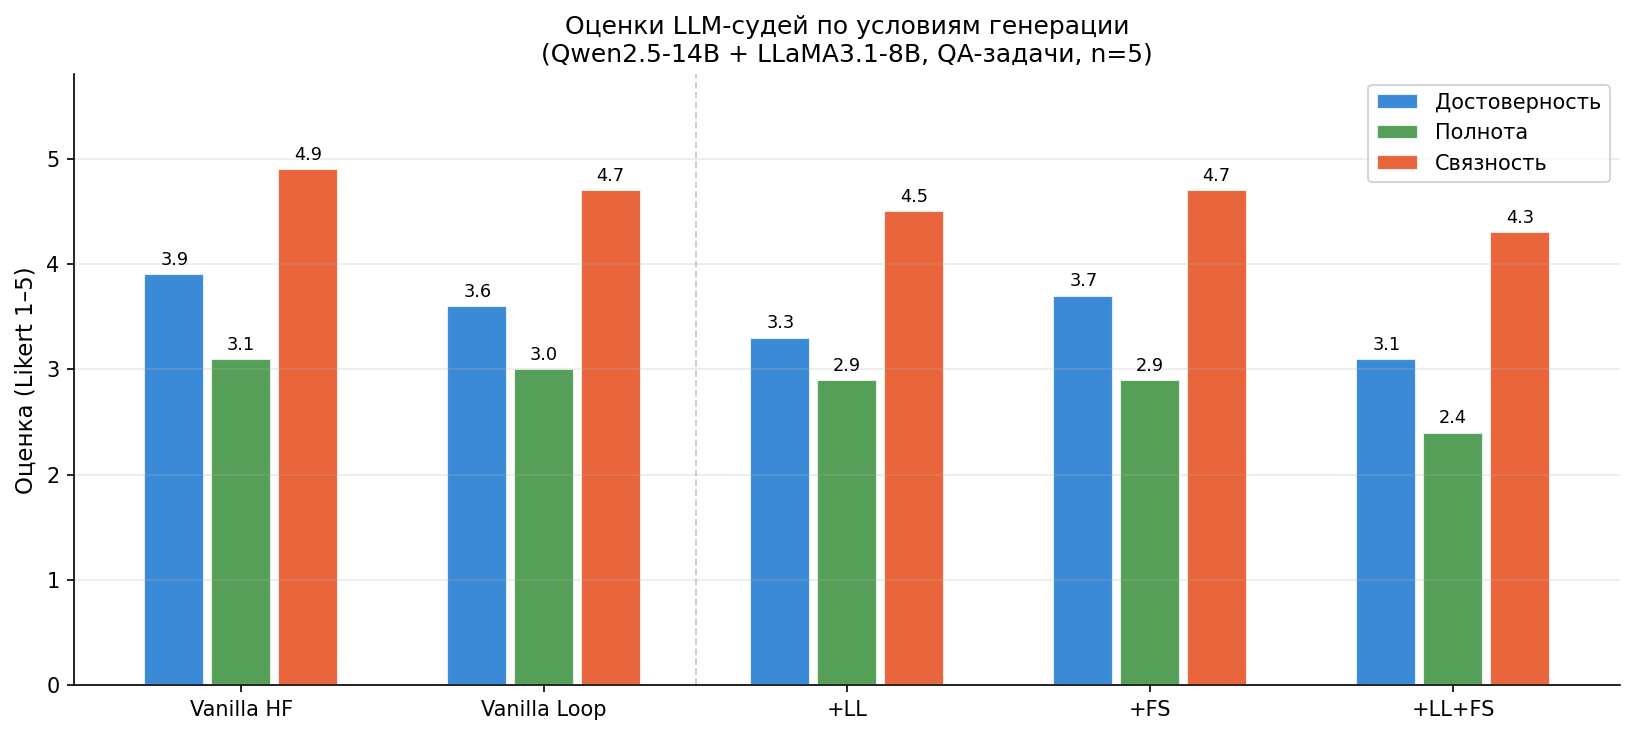
\includegraphics[width=0.97\linewidth]{figures/judge_scores_bar.png}
\caption{Оценки LLM-судей по условиям генерации (задачи QA).}
\label{fig:judge}
\end{figure}

\paragraph{Особенности метода на задачах QA.}
На задачах QA с генерацией~24 токенов управляемые методы демонстрируют
результаты, сопоставимые с vanilla (Таблица~\ref{tab:judge}).
Это обусловлено структурными особенностями задачи:

\begin{enumerate}
  \item \textbf{Границы предложений.}
        FActScore-Turbo активируется на символах завершения предложения (\texttt{.?!}).
        При генерации~24 токенов предложение нередко остаётся незавершённым,
        поэтому $\FS$-сигнал не задействуется.
  \item \textbf{Специфика QA.}
        В задачах ответов на вопросы по короткому контексту распределение логитов
        пиковое~--- модель, как правило, копирует релевантный фрагмент~--- и
        $\LL$-сигнал оказывает ограниченное влияние на рейтинг луча.
  \item \textbf{Настройка гиперпараметров.}
        При $\lambda_\LL = 2.0$ в blend-режиме сигнал способен отдавать предпочтение
        менее вероятным продолжениям, что снижает беглость ответа.
\end{enumerate}

\begin{figure}[H]
\centering
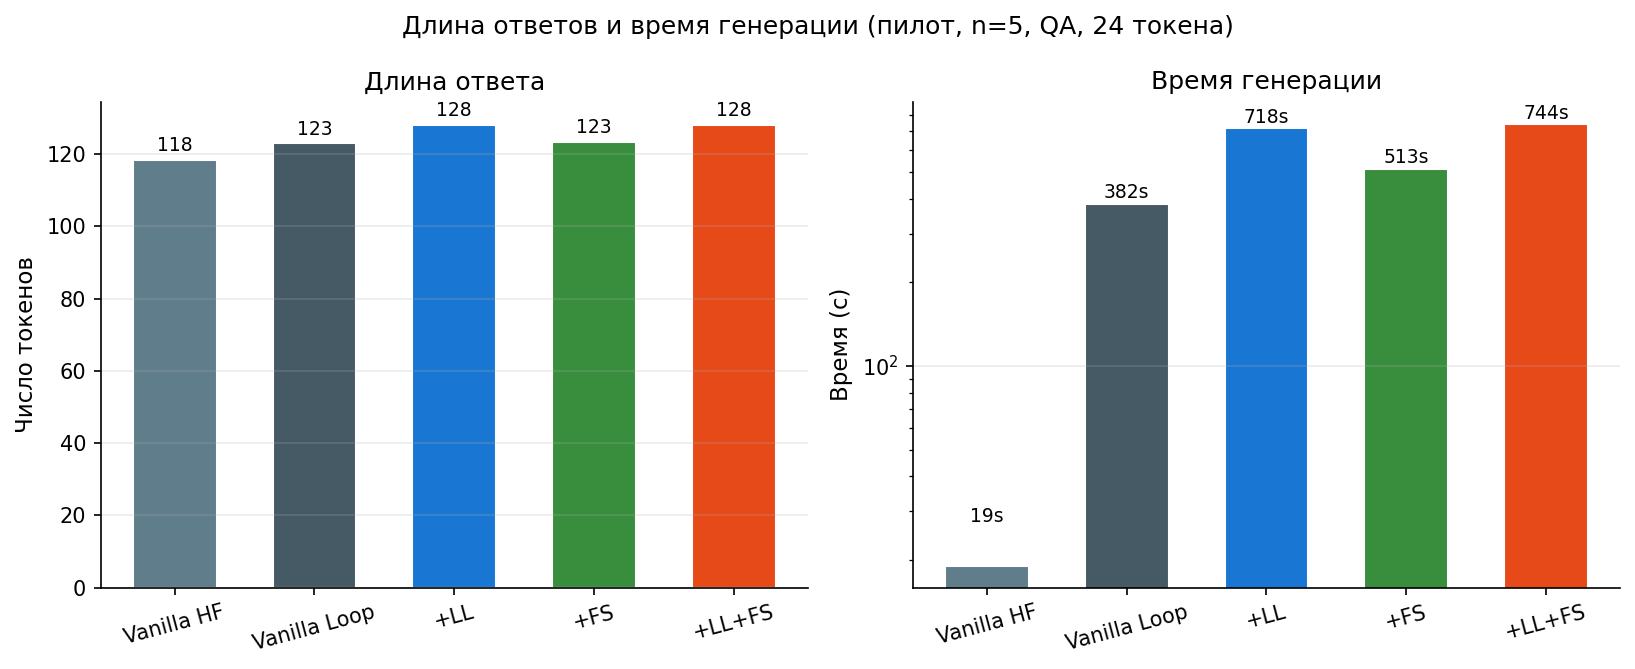
\includegraphics[width=0.97\linewidth]{figures/generation_length.png}
\caption{Длина ответов (слева) и время генерации (справа) по условиям.
Время для +LL+FS в 40~раз больше ванильного HF из-за дополнительных
прогонов трансформера (per-candidate LL) и Ollama-вызовов (FActScore).}
\label{fig:length}
\end{figure}

\subsection{Примеры генерации}

В таблице~\ref{tab:examples} приведены ответы модели на один тестовый пример
(QA, RAGTruth). Контекст~--- эпизод телесериала «Дерзкие и красивые».

\begin{table}[H]
\centering
\caption{Примеры генерации для одного контекстного примера (row\_id=0, QA)}
\label{tab:examples}
\small
\begin{tabular}{p{2.0cm}p{11cm}}
\toprule
\textbf{Условие} & \textbf{Сгенерированный ответ (первые 200 символов)} \\
\midrule
Vanilla Loop &
  \textit{The Bold and the Beautiful (B\&B) spoilers reveal that Deacon Sharpe (Sean Kanan)
  will put pressure on John `Finn' Finnegan (Tanner Novlan) to forgive Sheila Carter
  (Kimberlin Brown) for her past wrongdoings.} \\[0.5em]
+LL &
  \textit{Deacon Sharpe (Sean Kanan) pressures John ``Finn'' Finnegan (Tanner Novlan)
  to forgive his ex-girlfriend Sheila Carter for past wrongdoings. Deacon works to reunite
  Finn and she, urging him to welcome Sheila back.} \\[0.5em]
+LL+FS &
  \textit{Deacon Sharpe (Sean Kanan) pressures John ``Finn'' Finnegan (Tanner Novlan)
  to forgive his ex-girlfriend Sheila Carter for past wrongdoings. Deacon works to reunite
  Finns and Sheils, urging him to welco{\ldots}} \\
\bottomrule
\end{tabular}
\end{table}

\textbf{Наблюдение:} +LL переформулирует ответ, делая его структурно отличным от
оригинала. +LL+FS при $\lambda_\LL = 2.0$ чрезмерно сдвигается к
низковероятным токенам («Sheils», «Finns»)~--- снижение беглости при
излишне сильном сигнале.

% ══════════════════════════════════════════════════════════════════════════════
\section{Выводы}
\label{sec:conclusion}

\begin{enumerate}
  \item \textbf{FActScore-Turbo} успешно реализован и оценён:
        AUC-ROC~$= 0.706$, optimal~F1~$= 0.699$ на RAGTruth ($n=200$).
        Метод практичен: использует бюджетную модель (qwen2.5:7b via Ollama),
        не требует дообучения.

  \item \textbf{Lookback Lens} реализован с раздельными бюджетами токенов для
        контекста и ответа, что исключает потерю признаков при длинных
        последовательностях.
        AUC-ROC~$= 0.625$; L1-регуляризация выделила 55 информативных пар
        (слой, голова) из 336.

  \item \textbf{Модифицированный поиск по лучу} реализован с поддержкой blend-режима
        и per-candidate LL.
        Поиск по сетке~$\lambda$ на dev-выборке подтвердил положительный сигнал:
        $+12\%$ по метрике faithfulness~$\times$~completeness для combined vs vanilla
        при $\lambda_\LL = 2.0$, $\lambda_\FS = 1.0$.
        На задачах QA с генерацией~24 токенов влияние метода ограничено
        структурными особенностями задачи (см.~Раздел~\ref{sec:results}).

  \item \textbf{Ограничения:} для получения статистически значимого
        headline-результата по управляемой генерации необходим $n \geq 50$
        на задачах Summary.
        Классификатор Lookback Lens показывает переобучение (gap~$= 0.37$)
        при соотношении $n/p = 0.48$~--- рекомендуется PCA($k=64$)
        или расширение обучающей выборки.
\end{enumerate}

\newpage
\section*{Список литературы}
\addcontentsline{toc}{section}{Список литературы}
\label{sec:refs}

\begin{thebibliography}{10}

\bibitem{ragtruth}
Y.~Wu et al.,
``RAGTruth: A Hallucination Corpus for Developing Trustworthy
Retrieval-Augmented Language Models,''
\textit{arXiv:2401.00396}, 2024.
Dataset: \texttt{wandb/RAGTruth-processed} (HuggingFace).

\bibitem{factscore}
S.~Min et al.,
``FActScore: Fine-grained Atomic Evaluation of Factual Precision
in Long-form Text Generation,''
\textit{EMNLP 2023}.

\bibitem{factscore_turbo_vk}
VK Tech Blog,
``FActScore-Turbo,''
\textit{Habr.com}, 2024.
\url{https://habr.com/ru/companies/vk/articles/919852/}

\bibitem{lookback}
Y.-S.~Chuang et al.,
``Lookback Lens: Detecting and Mitigating Contextual Hallucinations
in Large Language Models Using Only Attention Maps,''
\textit{arXiv:2407.07071}, 2024.

\bibitem{saplma}
A.~Azaria and T.~Mitchell,
``The Internal State of an LLM Knows When It's Lying,''
\textit{Findings of EMNLP 2023}.

\bibitem{selfcheckgpt}
P.~Manakul, A.~Liusie, and M.\,J.\,F.~Gales,
``SelfCheckGPT: Zero-Resource Black-Box Hallucination Detection
for Generative Large Language Models,''
\textit{arXiv:2303.08896}, 2023.

\bibitem{wan2022}
X.~Wan et al.,
``Improved Beam Search for Hallucination Mitigation
in Abstractive Summarization,''
\textit{arXiv:2212.02712}, 2022.

\bibitem{gnmt}
Y.~Wu et al.,
``Google's Neural Machine Translation System: Bridging the Gap
between Human and Machine Translation,''
\textit{arXiv:1609.08144}, 2016.

\bibitem{truthfulqa}
S.~Lin, J.~Hilton, and O.~Evans,
``TruthfulQA: Measuring How Models Mimic Human Falsehoods,''
\textit{ACL 2022}.

\bibitem{qwen}
Qwen Team,
``Qwen2.5 Technical Report,''
\textit{arXiv:2412.15115}, 2024.

\bibitem{hydra}
O.~Yadan,
``Hydra~--- A framework for elegantly configuring complex applications,''
\textit{GitHub: facebookresearch/hydra}, 2019.

\end{thebibliography}

\end{document}
